\documentclass{article}
\usepackage{ctex}
\usepackage{listings}
\usepackage{xcolor}
\usepackage{graphicx}

\title{深度学习与神经网络第二次课程项目}
\author{王逸群 19307110397}
\date{2022.4.9}

\definecolor{gray}{rgb}{0.99,0.99,0.99}

\lstdefinestyle{mystyle}{
	basicstyle=\footnotesize,
	backgroundcolor=\color{gray},
	numbers=left
}

\lstset{style=mystyle}

\begin{document}
	
\maketitle
\tableofcontents

\section{神经网络}

\subsection{初始设置}

本项目使用CIFAR-10数据集,
其中包含60000张$32\times32$的彩色图片,
被平均分为10类:飞机、汽车、鸟、猫、鹿、狗、青蛙、马、船、货车。

参考VGG网络架构,
基于pytorch框架,
设计神经网络初始架构。
对于输入的图像,
先进行两轮卷积、激活、池化操作,
使图像边长由32变为16再变为8,
图像频道数由3变为16再变为32;
接着进行三轮线性、激活操作,
使神经元数量由$32\times8\times8$变为128再变为10。
初始架构的参数数量为285162,
类存储于\verb|Code/nn.py|,
具体内容如下:

\begin{lstlisting}[language=Python]
class NN(nn.Module):
    def __init__(self, in_channels = 3, hidden_channels = (16, 32), 
                 hidden_neurons = (128, 128), num_classes = 10):
        super().__init__()
        self.hidden_channels = hidden_channels

        self.extractor = nn.Sequential(
            # stage 1
            nn.Conv2d(in_channels = in_channels,
                      out_channels = hidden_channels[0],
                      kernel_size = 3, padding = 1),
            nn.ReLU(),
            nn.MaxPool2d(kernel_size = 2, stride = 2),

            # stage 2
            nn.Conv2d(in_channels = hidden_channels[0],
                      out_channels = hidden_channels[1],
                      kernel_size = 3, padding = 1),
            nn.ReLU(),
            nn.MaxPool2d(kernel_size = 2, stride = 2))

        self.classifier = nn.Sequential(
            nn.Linear(hidden_channels[1] * 8 * 8, hidden_neurons[0]),
            nn.ReLU(),
            nn.Linear(hidden_neurons[0], hidden_neurons[1]),
            nn.ReLU(),
            nn.Linear(hidden_neurons[1], num_classes))

    def forward(self, inputs):
        hidden = self.extractor(inputs)
        outputs = \
            self.classifier(hidden.view(-1,
                                        self.hidden_channels[1] * 8 * 8))
        return outputs
\end{lstlisting}

其余参数的初始设置如下:

损失函数:交叉熵损失函数;

优化器:Adam;

学习率:0.001;

初始设置运行结果如图\ref{fig:Original}所示,
训练集上的最优错误率为0.05860,在第19回合出现;
测试集上的最优错误率为0.30160,在第8回合出现。

\begin{figure}[h]
\includegraphics[width=\textwidth]
{Result/NN Original 0.001/figure.png}
\caption{原始模型在测试集和验证集上的错误率}
\label{fig:Original}
\end{figure}

\subsection{参数调整}

\subsubsection{神经元数量}

本节在总体架构不变的基础上,
改变神经元数量,
实验设置如表\ref{table:SizeSet}所示,
结果如表\ref{table:SizeResult}和图\ref{fig:Size}所示。

\begin{table}[h]
\centering
\begin{tabular}{|l|l|l|l|} 
\hline
& \verb|hidden_channels| & \verb|hidden_neurons| & 参数数量\\
\hline
原模型 & \verb|(16,  32)| & \verb|(128,  128)| & 285162 \\
更小的模型 & \verb|( 4,   8)| & \verb|( 32,   32)| & 18210 \\
更大的模型 & \verb|(64, 128)| & \verb|(512,  512)| & 4538250\\
\hline
\end{tabular}
\caption{神经元数量实验设置}
\label{table:SizeSet}
\end{table}

\begin{table}[h]
\centering
\begin{tabular}{|l|l|l|l|l|} 
\hline
& 训练集最优错误率 & 回合 & 测试集最优错误率 & 回合 \\
\hline
原模型 & 0.05860 & 19 & 0.30160 & 8 \\
更小的模型 & 0.37472 & 20 & 0.40570 & 20 \\
更大的模型 & 0.00978 & 19 & 0.26310 & 4 \\
\hline
\end{tabular}
\caption{神经元数量实验结果}
\label{table:SizeResult}
\end{table}

\begin{figure}[h]
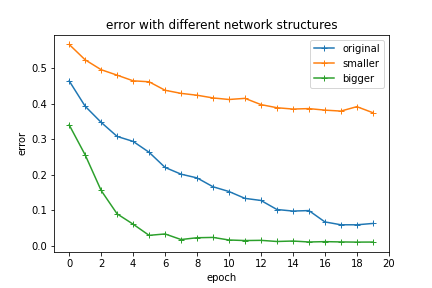
\includegraphics[width=\textwidth]
{Result/NN bigger/figure.png}
\caption{神经元数量实验结果}
\label{fig:Size}
\end{figure}

可以看到,随着模型的规模变大,参数数量增加,
训练集和测试集的最优错误率都有所上升,
但是测试集最优错误率的上升幅度非常有限。

\subsubsection{损失函数}

初始设置使用交叉熵损失函数,本节尝试使用多分类的合页损失函数。
实验结果如图\ref{fig:Loss}和表\ref{table:Loss}所示。

\begin{figure}[p]
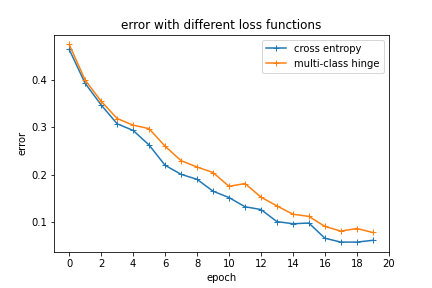
\includegraphics[width=\textwidth]
{Result/NN hinge/figure.png}
\caption{损失函数实验结果}
\label{fig:Loss}
\end{figure}

\begin{table}[h]
\centering
\begin{tabular}{|l|l|l|l|l|} 
\hline
损失函数 & 训练集最优错误率 & 回合 & 测试集最优错误率 & 回合 \\
\hline
交叉熵 & 0.05860 & 19 & 0.30160 & 8 \\
合页 & 0.07886 & 20 & 0.31200 & 15 \\
\hline
\end{tabular}
\caption{损失函数实验结果}
\label{table:Loss}
\end{table}

可以看到,使用多分类的合页损失函数并没有明显的提升效果。

\subsubsection{正则化}

初始设置未加入正则化,本节尝试使用不同的正则化参数,
实验结果如图\ref{fig:Regularize}和表\ref{table:Regularize}所示。

\begin{figure}[p]
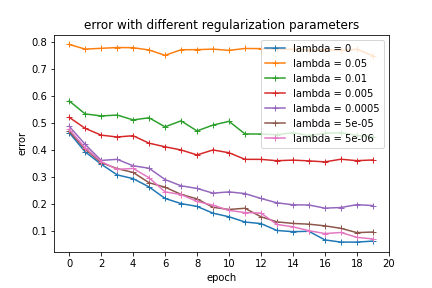
\includegraphics[width=\textwidth]
{Result/NN regularize 5e-06/figure.png}
\caption{正则化实验结果}
\label{fig:Regularize}
\end{figure}

\begin{table}[h]
\centering
\begin{tabular}{|l|l|l|l|l|} 
\hline
正则化参数 & 训练集最优错误率 & 回合 & 测试集最优错误率 & 回合 \\
\hline
0 & 0.05860 & 19 & 0.30160 & 8 \\
0.05 & 0.74906 & 20 & 0.74940 & 20 \\
0.01 & 0.45312 & 16 & 0.45140 & 20 \\
0.005 & 0.35582 & 17 & 0.37120 & 17 \\
0.0005 & 0.18448 & 17 & 0.30160 & 17 \\
0.00005 & 0.09378 & 19 & 0.31440 & 10 \\
0.000005 & 0.07034 & 20 & 0.31110 & 15 \\
\hline
\end{tabular}
\caption{正则化实验结果}
\label{table:Regularize}
\end{table}

可以看到,
正则化并不能提升结果,
可能的原因是初始模型并没有出现严重的过拟合现象。

\subsubsection{激活函数}

初始设置使用ReLU激活函数,本节尝试使用tanh和softplus激活函数。
实验结果如图\ref{fig:Activation}和表\ref{table:Activation}所示。

\begin{figure}[p]
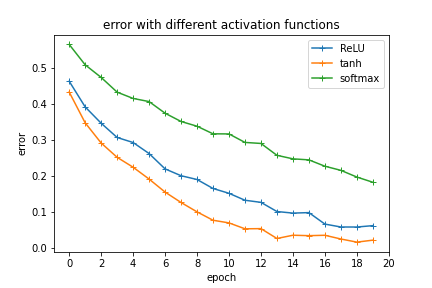
\includegraphics[width=\textwidth]
{Result/NN softplus/figure.png}
\caption{激活函数实验结果}
\label{fig:Activation}
\end{figure}

\begin{table}[h]
\centering
\begin{tabular}{|l|l|l|l|l|} 
\hline
激活函数 & 训练集最优错误率 & 回合 & 测试集最优错误率 & 回合 \\
\hline
ReLU & 0.05860 & 19 & 0.30160 & 8 \\
tanh & 0.01660 & 19 & 0.31510 & 8 \\
softplus & 0.18318 & 20 & 0.36490 & 14 \\
\hline
\end{tabular}
\caption{激活函数实验结果}
\label{table:Activation}
\end{table}

可以看到,
在训练集上,tanh激活函数的效果优于ReLU,softplus最次;
但在测试集上,ReLU表现最优。

\subsubsection{优化器}

初始设置使用Adam优化器,
本节尝试使用随机梯度下降优化器、
带有动量的随机梯度下降优化器、
以及Adagrad优化器,
实验结果如图\ref{fig:Optimize}和表\ref{table:Optimize}所示。

\begin{figure}[p]
\includegraphics[width=\textwidth]
{Result/NN Adagrad/figure.png}
\caption{优化器实验结果}
\label{fig:Optimize}
\end{figure}

\begin{table}[h]
\centering
\begin{tabular}{|l|l|l|l|l|} 
\hline
优化器 & 训练集最优错误率 & 回合 & 测试集最优错误率 & 回合 \\
\hline
Adam & 0.05860 & 19 & 0.30160 & 8 \\
SGD & 0.78832 & 20 & 0.78390 & 20 \\
Momentum & 0.36856 & 20 & 0.39020 & 20 \\
Adagrad & 0.23366 & 20 & 0.31240 & 18 \\
\hline
\end{tabular}
\caption{优化器实验结果}
\label{table:Optimize}
\end{table}

可以看到,初始设置的Adam优化器效果最优。

\subsubsection{批归一化}

本节尝试使用批归一化,
实验结果如图\ref{fig:BN}和表\ref{table:BN}所示。

\begin{figure}[p]
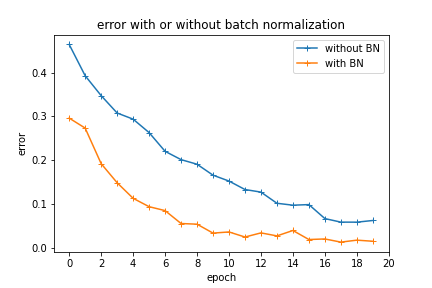
\includegraphics[width=\textwidth]
{Result/NN BN 0.001/figure.png}
\caption{批归一化实验结果}
\label{fig:BN}
\end{figure}

\begin{table}[h]
\centering
\begin{tabular}{|l|l|l|l|l|} 
\hline
批归一化 & 训练集最优错误率 & 回合 & 测试集最优错误率 & 回合 \\
\hline
否 & 0.05860 & 19 & 0.30160 & 8 \\
是 & 0.01306 & 18 & 0.29240 & 5 \\
\hline
\end{tabular}
\caption{批归一化实验结果}
\label{table:BN}
\end{table}

可以看到,
批归一化很好地提升了模型的效果,
但是测试集最优错误率的上升幅度非常有限。

\subsubsection{丢弃法}

本节尝试使用丢弃法,
实验结果如图\ref{fig:dropout}和表\ref{table:dropout}所示。

\begin{figure}[p]
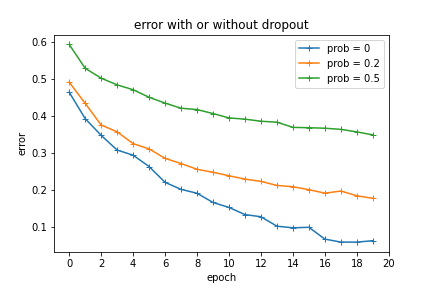
\includegraphics[width=\textwidth]
{Result/NN dropout 0.5/figure.png}
\caption{丢弃法实验结果}
\label{fig:dropout}
\end{figure}

\begin{table}[h]
\centering
\begin{tabular}{|l|l|l|l|l|} 
\hline
丢弃概率 & 训练集最优错误率 & 回合 & 测试集最优错误率 & 回合 \\
\hline
0 & 0.05860 & 19 & 0.30160 & 8 \\
0.2 & 0.17718 & 20 & 0.30560 & 20 \\
0.5 & 0.34874 & 20 & 0.38150 & 20 \\
\hline
\end{tabular}
\caption{丢弃法实验结果}
\label{table:dropout}
\end{table}

可以看到,丢弃法使得收敛速度变慢,无法提升模型效果。

\subsection{最优设置}

最终选择的最优设置是带有批归一化的模型.
对于输入的图像,
先进行两轮卷积、批归一化、激活、池化操作,
使图像边长由32变为16再变为8,
图像频道数由3变为16再变为32;
接着进行三轮线性、批归一化、激活操作,
使神经元数量由$32\times8\times8$变为128再变为10。
参数数量为285770,
类存储于\verb|Code/nn.py|,
具体内容如下:

\begin{lstlisting}[language=Python]
class NN_BN(nn.Module):
    def __init__(self, in_channels = 3, hidden_channels = (16, 32),
                 hidden_neurons = (128, 128), num_classes = 10):
        super().__init__()
        self.hidden_channels = hidden_channels

        self.extractor = nn.Sequential(
            # stage 1
            nn.Conv2d(in_channels = in_channels,
                      out_channels = hidden_channels[0],
                      kernel_size = 3, padding = 1),
            nn.BatchNorm2d(hidden_channels[0]),
            nn.ReLU(),
            nn.MaxPool2d(kernel_size = 2, stride = 2),

            # stage 2
            nn.Conv2d(in_channels = hidden_channels[0],
                      out_channels = hidden_channels[1],
                      kernel_size = 3, padding = 1),
            nn.BatchNorm2d(hidden_channels[1]),
            nn.ReLU(),
            nn.MaxPool2d(kernel_size = 2, stride = 2))

        self.classifier = nn.Sequential(
            nn.Linear(hidden_channels[1] * 8 * 8, hidden_neurons[0]),
            nn.BatchNorm1d(hidden_neurons[0]),
            nn.ReLU(),
            nn.Linear(hidden_neurons[0], hidden_neurons[1]),
            nn.BatchNorm1d(hidden_neurons[1]),
            nn.ReLU(),
            nn.Linear(hidden_neurons[1], num_classes))

    def forward(self, inputs):
        hidden = self.extractor(inputs)
        outputs = \
            self.classifier(hidden.view(-1,
                                        self.hidden_channels[1] * 8 * 8))
        return outputs
\end{lstlisting}

实验结果如图\ref{fig:BN}和表\ref{table:BN}所示,
另可视化Loss Landscape如图\ref{fig:NNLL}所示。

\begin{figure}[h]
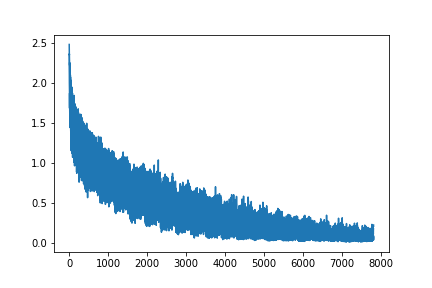
\includegraphics[width=\textwidth]
{Result/NN BN 0.0005/figure.png}
\caption{Loss Landscape}
\label{fig:NNLL}
\end{figure}

可以看到,批归一化很好地提升了模型的效果。

\section{VGG网络}

本项目同样使用CIFAR-10数据集。

参考VGG网络架构,
设计不带有批归一化的VGG网络和带有批归一化的VGG网络,
类存储于\verb|Code/vgg.py|,
具体内容如下:

\begin{lstlisting}[language=python]
class VGG(nn.Module):
    def __init__(self, in_channels = 3, num_classes = 10):
        super().__init__()

        self.extractor = nn.Sequential(
            # stage 1
            nn.Conv2d(in_channels = in_channels, out_channels = 64, 
                      kernel_size = 3, padding = 1),
            nn.ReLU(),
            nn.MaxPool2d(kernel_size = 2, stride = 2),

            # stage 2
            nn.Conv2d(in_channels = 64, out_channels = 128, 
                      kernel_size = 3, padding = 1),
            nn.ReLU(),
            nn.MaxPool2d(kernel_size = 2, stride = 2),

            # stage 3
            nn.Conv2d(in_channels = 128, out_channels = 256, 
                      kernel_size = 3, padding = 1),
            nn.ReLU(),
            nn.Conv2d(in_channels = 256, out_channels = 256, 
                      kernel_size = 3, padding = 1),
            nn.ReLU(),
            nn.MaxPool2d(kernel_size = 2, stride = 2),

            # stage 4
            nn.Conv2d(in_channels = 256, out_channels = 512, 
                      kernel_size = 3, padding = 1),
            nn.ReLU(),
            nn.Conv2d(in_channels = 512, out_channels = 512, 
                      kernel_size = 3, padding = 1),
            nn.ReLU(),
            nn.MaxPool2d(kernel_size = 2, stride = 2),

            # stage5
            nn.Conv2d(in_channels = 512, out_channels = 512, 
                      kernel_size = 3, padding = 1),
            nn.ReLU(),
            nn.Conv2d(in_channels = 512, out_channels = 512, 
                      kernel_size = 3, padding = 1),
            nn.ReLU(),
            nn.MaxPool2d(kernel_size = 2, stride = 2))

        self.classifier = nn.Sequential(
            nn.Linear(512 * 1 * 1, 512),
            nn.ReLU(),
            nn.Linear(512, 512),
            nn.ReLU(),
            nn.Linear(512, num_classes))

    def forward(self, inputs):
        hidden = self.extractor(inputs)
        outputs = self.classifier(hidden.view(-1, 512 * 1 * 1))
        return outputs


class VGG_BN(nn.Module):
    def __init__(self, in_channels = 3, num_classes = 10):
        super().__init__()

        self.extractor = nn.Sequential(
            # stage 1
            nn.Conv2d(in_channels = in_channels, out_channels = 64, 
                      kernel_size = 3, padding = 1),
            nn.BatchNorm2d(64),
            nn.ReLU(),
            nn.MaxPool2d(kernel_size = 2, stride = 2),

            # stage 2
            nn.Conv2d(in_channels = 64, out_channels = 128, 
                      kernel_size = 3, padding = 1),
            nn.BatchNorm2d(128),
            nn.ReLU(),
            nn.MaxPool2d(kernel_size = 2, stride = 2),

            # stage 3
            nn.Conv2d(in_channels = 128, out_channels = 256, 
                      kernel_size = 3, padding = 1),
            nn.BatchNorm2d(256),
            nn.ReLU(),
            nn.Conv2d(in_channels = 256, out_channels = 256, 
                      kernel_size = 3, padding = 1),
            nn.BatchNorm2d(256),
            nn.ReLU(),
            nn.MaxPool2d(kernel_size = 2, stride = 2),

            # stage 4
            nn.Conv2d(in_channels = 256, out_channels = 512, 
                      kernel_size = 3, padding = 1),
            nn.BatchNorm2d(512),
            nn.ReLU(),
            nn.Conv2d(in_channels = 512, out_channels = 512, 
                      kernel_size = 3, padding = 1),
            nn.BatchNorm2d(512),
            nn.ReLU(),
            nn.MaxPool2d(kernel_size = 2, stride = 2),

            # stage5
            nn.Conv2d(in_channels = 512, out_channels = 512, 
                      kernel_size = 3, padding = 1),
            nn.BatchNorm2d(512),
            nn.ReLU(),
            nn.Conv2d(in_channels = 512, out_channels = 512, 
                      kernel_size = 3, padding = 1),
            nn.BatchNorm2d(512),
            nn.ReLU(),
            nn.MaxPool2d(kernel_size = 2, stride = 2))

        self.classifier = nn.Sequential(
            nn.Linear(512 * 1 * 1, 512),
            nn.BatchNorm2d(512),
            nn.ReLU(),
            nn.Linear(512, 512),
            nn.BatchNorm2d(512),
            nn.ReLU(),
            nn.Linear(512, num_classes))

    def forward(self, inputs):
        hidden = self.extractor(inputs)
        outputs = self.classifier(hidden.view(-1, 512 * 1 * 1))
        return outputs
\end{lstlisting}
	
实验结果如图\ref{fig:VGG}和表\ref{table:VGG}所示,
另可视化Loss Landscape如图\ref{fig:VGGLL}所示。

\begin{table}[h]
\centering
\begin{tabular}{|l|l|l|l|l|} 
\hline
批归一化 & 训练集最优错误率 & 回合 & 测试集最优错误率 & 回合 \\
\hline
否 & 0.02462 & 19 & 0.25190 & 20 \\
是 & 0.01004 & 20 & 0.17030 & 16 \\
\hline
\end{tabular}
\caption{VGG网络实验结果}
\label{table:VGG}
\end{table}

\begin{figure}[h]
\includegraphics[width=\textwidth]
{Result/VGG BN 0.001/figure.png}
\caption{VGG网络实验结果}
\label{fig:VGG}
\end{figure}

\begin{figure}[h]
\includegraphics[width=\textwidth]
{Result/VGG BN 0.0005/figure.png}
\caption{Loss Landscape}
\label{fig:VGGLL}
\end{figure}

可以看到,
虽然使用批归一化对训练集最优错误率的提升很有限,
它很好地提升了测试集最优错误率,并加快了收敛速度。

\end{document}